\documentclass{report}
\usepackage[T1]{fontenc} % Fontes T1
\usepackage[utf8]{inputenc} % Input UTF8
\usepackage[backend=biber, style=ieee]{biblatex} % para usar bibliografia
\usepackage{csquotes}
\usepackage[portuguese]{babel} %Usar língua portuguesa
\usepackage{blindtext} % Gerar texto automaticamente
\usepackage[printonlyused]{acronym}
\usepackage{hyperref} % para autoref
\usepackage{graphicx}
\usepackage{titlesec}

\bibliography{bibliografia}


\begin{document}
%%
% Definições
%
\def\titulo{Projeto 2: Biblioteca de imagens}
\def\data{08/05/2019}
\def\autores{André Patacas, Gil Teixeira, Sofia Vaz, Luis Andrade}
\def\autorescontactos{(93357) andrepatacas@ua.pt, (88194) gilteixeira@ua.pt, (92968) sofiateixeiravaz@ua.pt, (93159) luisnunoferreirap.a@ua.pt}
\def\versao{1}
\def\departamento{DETI}
\def\empresa{LABI}
\def\logotipo{ua.pdf}

%
%%%%%% CAPA %%%%%%
%
\begin{titlepage}

\begin{center}
\centering
%
\vspace*{50mm}
%
{\Huge \titulo}\\ 
%
\vspace{10mm}
%
{\Large \empresa}\\
%
\vspace{10mm}
%
{\large \autores}\\ 
%
\vspace{30mm}
%
\begin{figure}[h]
\centering
\includegraphics{\logotipo}
\end{figure}
%
\vspace{30mm}
\end{center}
%
\begin{flushright}
\versao
\end{flushright}
\end{titlepage}

%%  Página de Título %%
\title{%
{\Huge\textbf{\titulo}}\\
{\Large \departamento\\ \empresa}
}
%
\author{%
    \autores 
}
%
\date{\data}
%
\maketitle


\pagenumbering{roman}

%%%%%% RESUMO %%%%%%
\begin{abstract}
Este relatório pretende descrever como uma biblioteca de imagens pesquisável foi desenvolvida no âmbito da cadeira de Laboratório de Informática. Esta biblioteca de imagens foi feita com base em Python 3, \ac{CSS}, JavaScript e \ac{HTML}. Neste relatório incluímos a divisão geral do trabalho, a explicação geral de métodos criados no \textit{backend} e \textit{frontend} e imagens dos resultados. 
\end{abstract}

%%%%%% Agradecimentos %%%%%%
% Segundo glisc deveria aparecer após conclusão...

\tableofcontents
 \listoftables     % descomentar se necessário
 \listoffigures    % descomentar se necessário


%%%%%%%%%%%%%%%%%%%%%%%%%%%%%%%
\clearpage
\pagenumbering{arabic}

%%%%%%%%%%%%%%%%%%%%%%%%%%%%%%%%
\chapter{Introdução}
\label{chap.introducao}

O frontend da aplicação foi feito em \ac{HTML}, \ac{CSS} e JavaScript e o backend foi feito em Python 3. Esta aplicação foi feita no âmbito de Laboratórios de Informática no ano letivo 2018/2019.
A adicionar às especificações básicas pedidas no o guião sobre regras do segundo projeto, construiu-se ainda suporte para pydocs e um sistema de pesquisa de imagens por qualquer cor do espectro rgb.
Este documento está dividido em quatro capítulos.
Depois desta introdução,
no \autoref{chap.metodologia} é apresentada a metodologia seguida, tendo em conta o trabalho faseado de cada um, 
no \autoref{chap.resultados} são apresentados os resultados obtidos,
sendo estes discutidos no \autoref{chap.analise}.
Finalmente, no \autoref{chap.conclusao} são apresentadas
as conclusões do trabalho.

\chapter{Metodologia}
\label{chap.metodologia}
\section{Definição de tarefas}
Esta fase consistiu em, antes de começar a trabalhar, definir quais membros do grupo fariam o quê, o que pode ser consultado na tabela \ref{tab:table1}: 
\begin{table}[h!]
\begin{center}
\caption{Divisão geral de tarefas}
\begin{tabular}{l|l}
\hline
\multicolumn{1}{|l|}{Aluno} & \multicolumn{1}{l|}{Tarefa Atribuída} \\ \hline
            André Patacas   & backend                               \\ 
            Gil Teixeira      & frontend                               \\
            Sofia Vaz         & relatório                                \\
            Luis Andrade    & testes unitários e funcionais                     
\end{tabular}
\label{tab:table1}
\end{center}
\end{table}

\section{Backend}
\subsection{DbCommunicator.py}
\paragraph{\_\_init\_\_}
Este método inicializa o objeto que comunica com a base de dados.

\paragraph{get\_dims\_and\_color}
Este método devolve os dados da imagem, a HUE da cor média e as dimensões. 

\paragraph{request\_caracteristics}
Este método liga-se ao \textit{website} fornecido pelos docentes, devolvendo um array em que cada elemento é um \ac{json} com:
\begin{itemize}
\item nome, que é o resultado do \textit{hashing} do conteúdo das imagens para evitar imagens replicadas
\item classe
\item \textit{bounding box}, ou seja, a área onde a classe se verifica
\item "confiança" com a qual o servidor conseguiu classificar a imagem
\end{itemize}

\paragraph{add}
Este método adiciona uma imagem à base de dados. Se uma imagem tiver várias classes será cortada, 
tendo cada parte uma classe diferente, sendo também guardada a original. A base de dados terá a 
seguinte informação para cada objeto:
\begin{itemize}
\item nome
\item altura
\item largura
\item quantidade média de vermelho
\item quantidade média de verde
\item quantidade média de azul
\item \textit{boundig box}
\item confiança, de 0 a 1, de que a imagem foi classificada corretamente
\end{itemize}

\paragraph{remove}
Ao executar este método, uma dada imagem e todas as suas associadas serão removidas da base de dados.

\paragraph{get}
Este método devolve informação sobre uma imagem indentificada pelo id fornecido como parâmetro.

\paragraph{request}

Devolve uma string com os dados pedidos no argumento. O funcionamento é analogo ao descrito no enunciado.


\paragraph{Setup}
Ambos os métodos \_\_clear\_all\_caution\_\_ e  populate são usados para efeitos de \textit{setup} inicial.

\subsection{app.py}
Este programa serve os conteúdos estáticos \ac{HTML}, JavaScript e \ac{CSS} e cria uma API transformando os GET e POST requests em chamadas de funções comunicantes com a base de dados. 

\subsection{put\_example}
Este programa envia uma imagem para a base de dados, não tendo qualquer efeito na maneira como o \textit{website} funciona.

\section{Frontend}
Para uma biblioteca de imagens ser viável, a compatibilidade entre dispositivos é necessária. Por isso, na criação desta, foi sempre tida em conta a usabilidade não só em monitores de computador, mas também em dispositivos móveis. 

\subsection{Home/Class List}
Esta página informa o utilizador de todas as classes já detetadas nesta biblioteca, mostrando alguns exemplos. Ao carregar no nome de uma classe, entra-se numa página em que todas as imagens da classe estão visíveis. Ao carregar numa imagem, o utilizador abre-a, vendo a imagem original e ainda as \textit{bounding boxes} de cada classe presente. O ficheiro de \ac{JS} associado é:
\paragraph{class\_list} 
Lista as classes já detetadas e apresenta imagens com exemplos.

\subsection{List Images}
\label{listimages}
Esta página mostra as imagens cortadas presentes na biblioteca sem nenhuma ordem em particular. Ao fazer \textit{hover} com o rato, é dada a informação sobre a classe detetada e a confiança com que foi classificada. Ao carregar no botão \textit{more}, é aberta a imagem numa nova pagina. Pode ver o código desta página no ficheiro list\_images.html. O ficheiro de \ac{JS} associado é:
\paragraph{image\_loader}
Mostra as imagens segundo os dados inseridos pelo utilizador. Pesquisará segundo a classe se dados forem inseridos dados na caixa de texto. Se a caixa de \textit{Class Detection Confidence} estiver \textit{ticked}, então apenas serão mostradas imagens com uma confiança igual ou superior à selecionada. Se a caixa \textit{Search with color} estiver ativa, então as imagens surgirão segundo a sua proximidade com a cor selecionada. A caixa \textit{Color Confidence} tem funcionamento parecido com a \textit{Class Detection Confidence}. Nesta página, como não há pesquisa integrada, apenas mostra as imagens.


\subsection{Send Image}
Dá a possibilidade ao utilizador de inserir as próprias imagens na biblioteca. Para adicionar estes dados, o utilizador pode abrir o explorador de ficheiros a partir do botão da página ou arrastar uma para o \textit{form}. Se uma classe for detetada, então a base de dados será atualizada com a informação da nova imagem e esta ficará acessível a todos os utilizadores da biblioteca. O ficheiro de \ac{JS} associado é:
\paragraph{send\_image}
Envia a imagem via POST request para o \textit{backend} do \textit{website}.

\subsection{Inspect Image}
Esta página mostra a imagem  com as \textit{bounding boxes} de cada classe, informando o utilizador o que cada caixa é. O ficheiro de \ac{JS} associado é:
\paragraph{image\_inspect}
Quando uma imagem é aberta, esta função mostra ao utilizador as \textit{bounding boxes} de cada classe e informação sobre estas. 


\subsection{Search Images}
Esta página apresenta o motor de busca da biblioteca. É possível pesquisar por classe e por cor. 
A pesquisa por classe é feita a partir de uma caixa de texto em que são introduzidos dados e a pesquisa por cor é feita a partir de um seletor de cor, tornando a experiência o mais intuitiva possível para o utilizador. Para além disso, é possível definir a confiança mínima na deteção da classe e cor. Os ficheiros de \ac{JS} associados são:
\paragraph{handlers}
Faz com que a página tenha uma seta no fundo para passar à página seguinte. Para além disso, faz com que o ficheiro image\_loader faça a procura segundo as caixas que estão \textit{ticked}.
\paragraph{image\_loader}
Este ficheiro foi explicado na \autoref{listimages}.

\subsection{About}
Aqui é possível encontrar os dados de todos os membros do grupo(nome, número mecanográfico, e-mail institucional) e a percentagem do trabalho feito por cada um.

\subsection{Pagina de Erro}
Esta página é mostrada quando ocorre um erro, desde tentativa de acesso a paginas que nao existem até erros internos.
Uma maneira de invocar um erro deste tipo é tentar aceder a imagens ou páginas que não existem. 


\chapter{Resultados}
\label{chap.resultados}
Nas imagens \ref{Fig1} e \ref{Fig2} é possível ver a página Class List, onde as classes detetadas até agora são listadas com alguns exemplos. Na imagem \ref{Fig3} é possível ver uma imagem aberta com as \textit{bounding boxes} (a azul) e a classe de cada \textit{bounding box} (a vermelho). Na imagem \ref{Fig4} é possível ver os dados que uma imagem mostra quando é feito \textit{hover} com o rato, sendo estes dados a classe da imagem e a confiança. Na imagem \ref{Fig5} vê-se a página List Images, sendo esta a página que lista todas as imagens sem nenhum critério de organização. Nas imagens \ref{Fig6}, \ref{Fig7} e \ref{Fig8} vê-se a página de pesquisa. Na primeira imagem a pesquisa não tem dados inseridos e na segunda procura-se por uma cor específica (preto). Na terceira procura-se uma classe específica (cão). Na imagem \ref{Fig9} está representada a página de sumbissão de imagens, sendo esta a página que possibilita a inserção de imagens por cada utilizador. Na figura \ref{Fig10} vê-se a página de inspeção de uma imagem com alguns GET requests associados.

\begin{figure}[h]
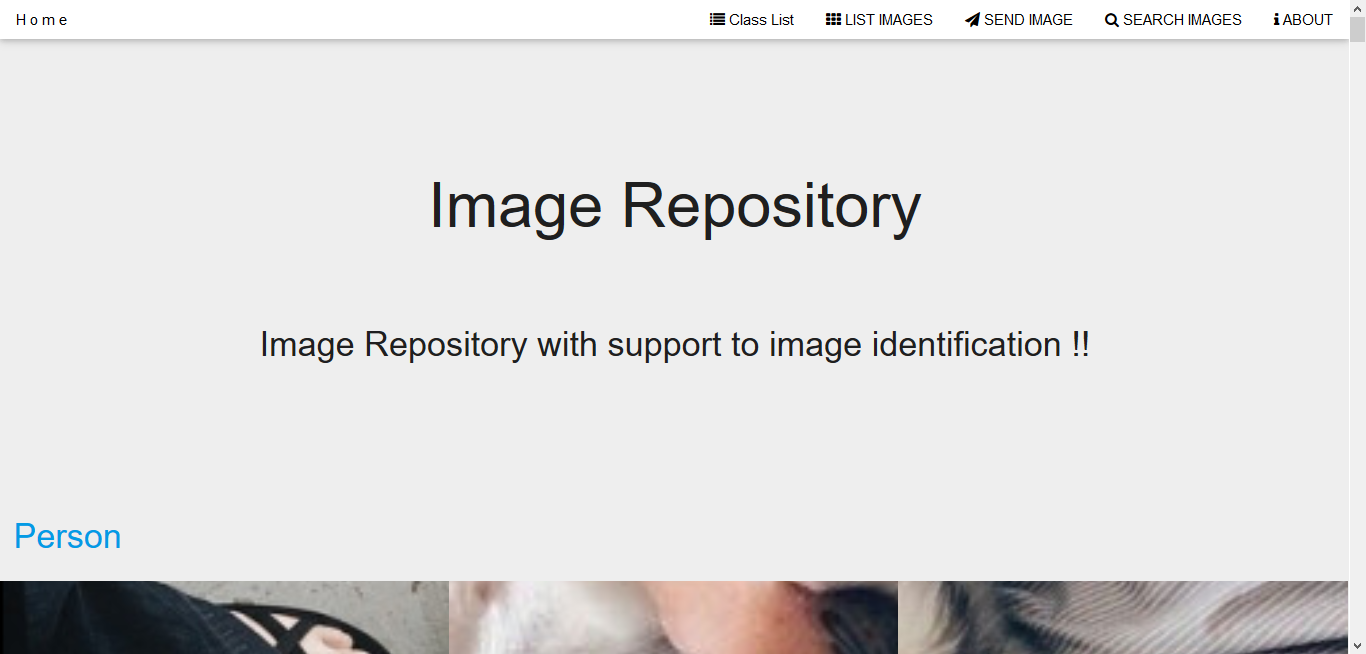
\includegraphics[width=\textwidth]{HomeTOP.png}
\caption{Topo da página Home/Class List}
\label{Fig1}
\end{figure}

\begin{figure}[h]
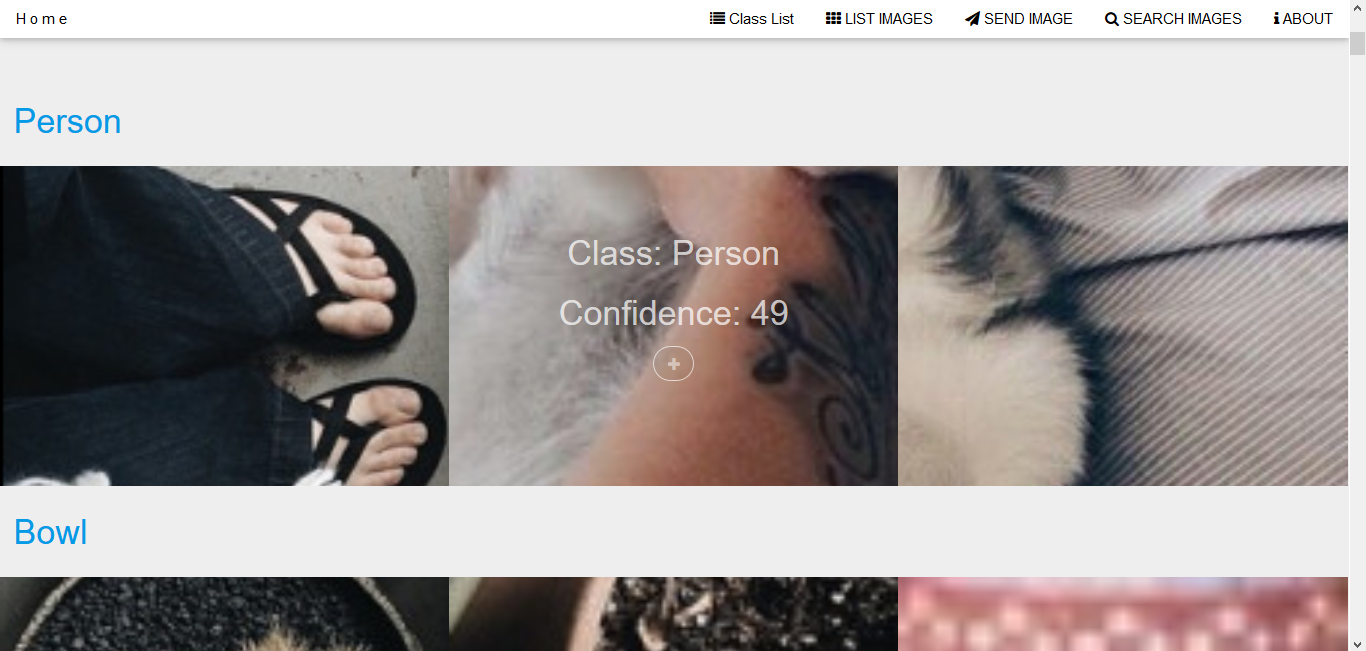
\includegraphics[width=\textwidth]{HomeBOTTOM.png}
\caption{Página Home/Class List com as imagens e classes visíveis}
\label{Fig2}
\end{figure}

\begin{figure}[h]
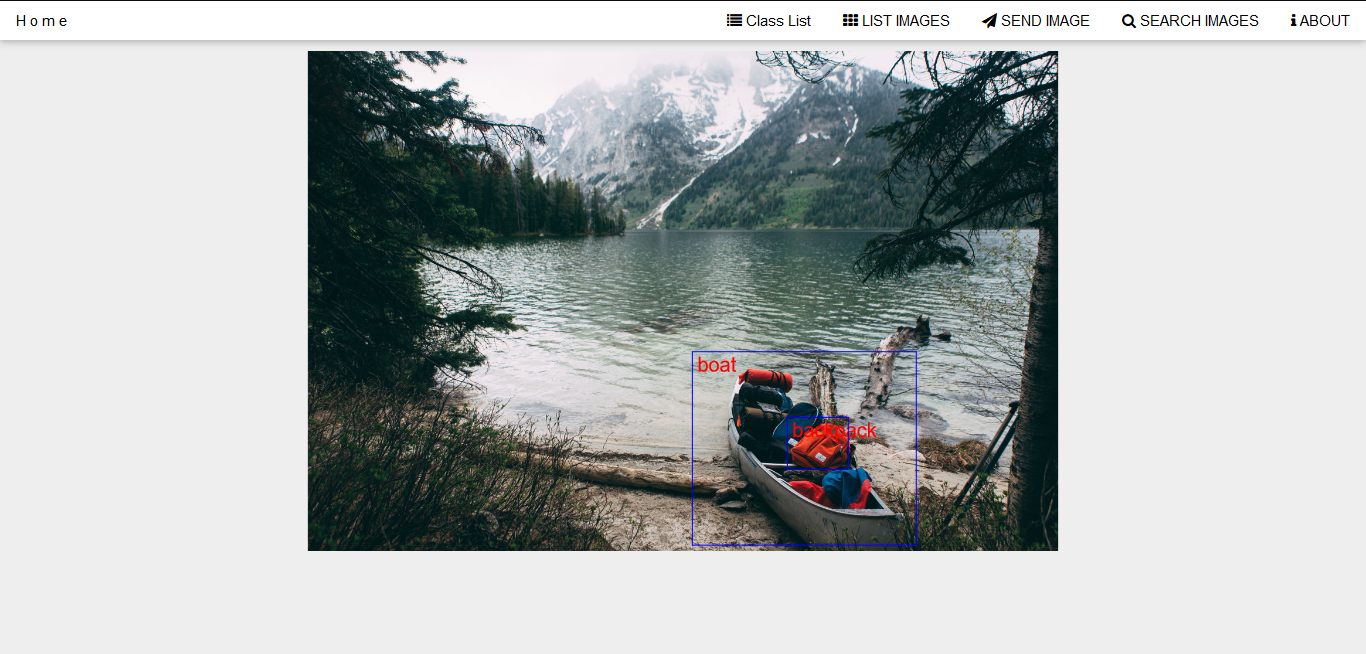
\includegraphics[width=\textwidth]{dataImage.png}
\caption{Dados de uma imagem aberta}
\label{Fig3}
\end{figure}

\begin{figure}[h]
\includegraphics[width=\textwidth]{ExemploHOVER.png}
\caption{Efeito \textit{hover} numa imagem}
\label{Fig4}
\end{figure}

\begin{figure}[h]
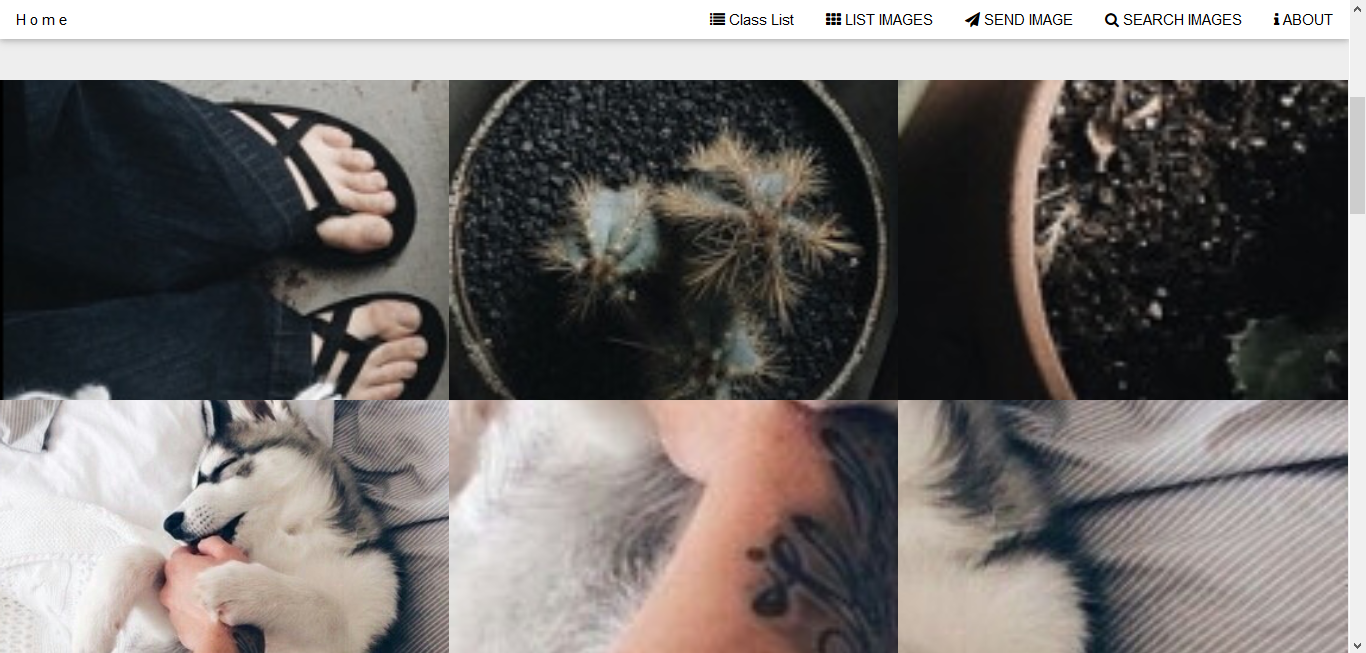
\includegraphics[width=\textwidth]{ListImages.png}
\caption{Página em que todas as imagens estão listadas}
\label{Fig5}
\end{figure}


\begin{figure}[h]
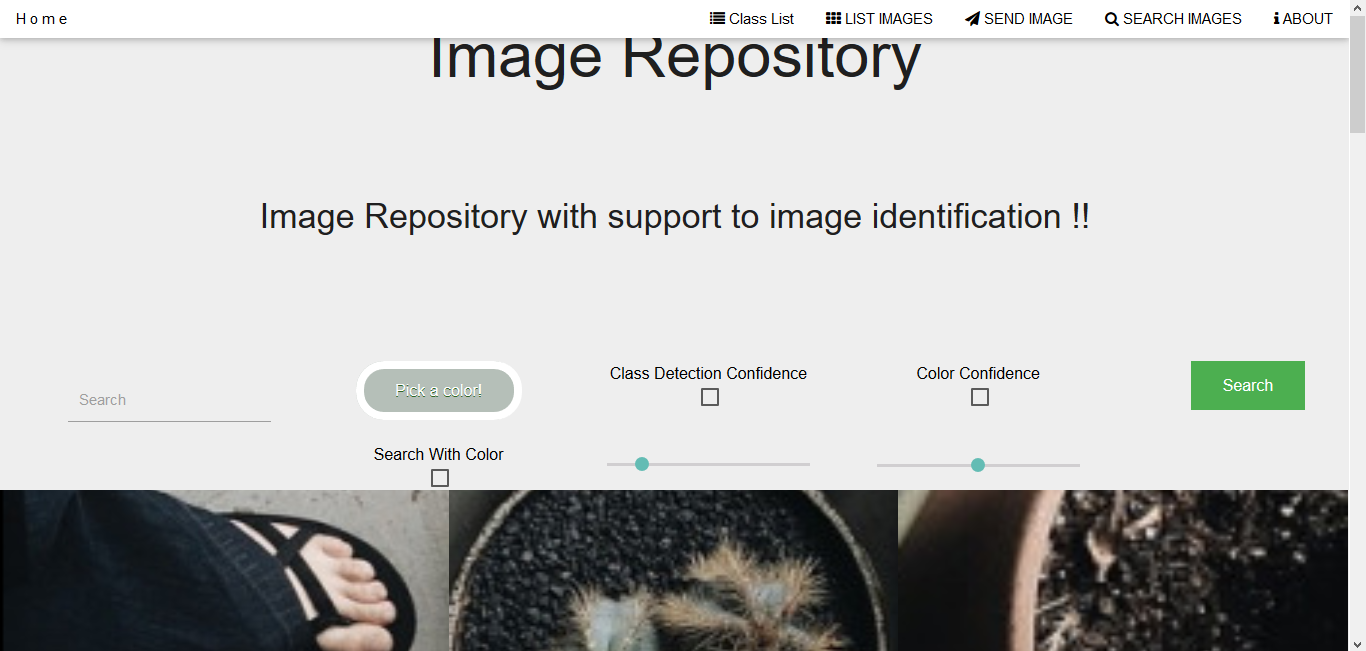
\includegraphics[width=\textwidth]{SearchDefault.png}
\caption{Página de pesquisa sem dados inseridos}
\label{Fig6}
\end{figure}

\begin{figure}[h]
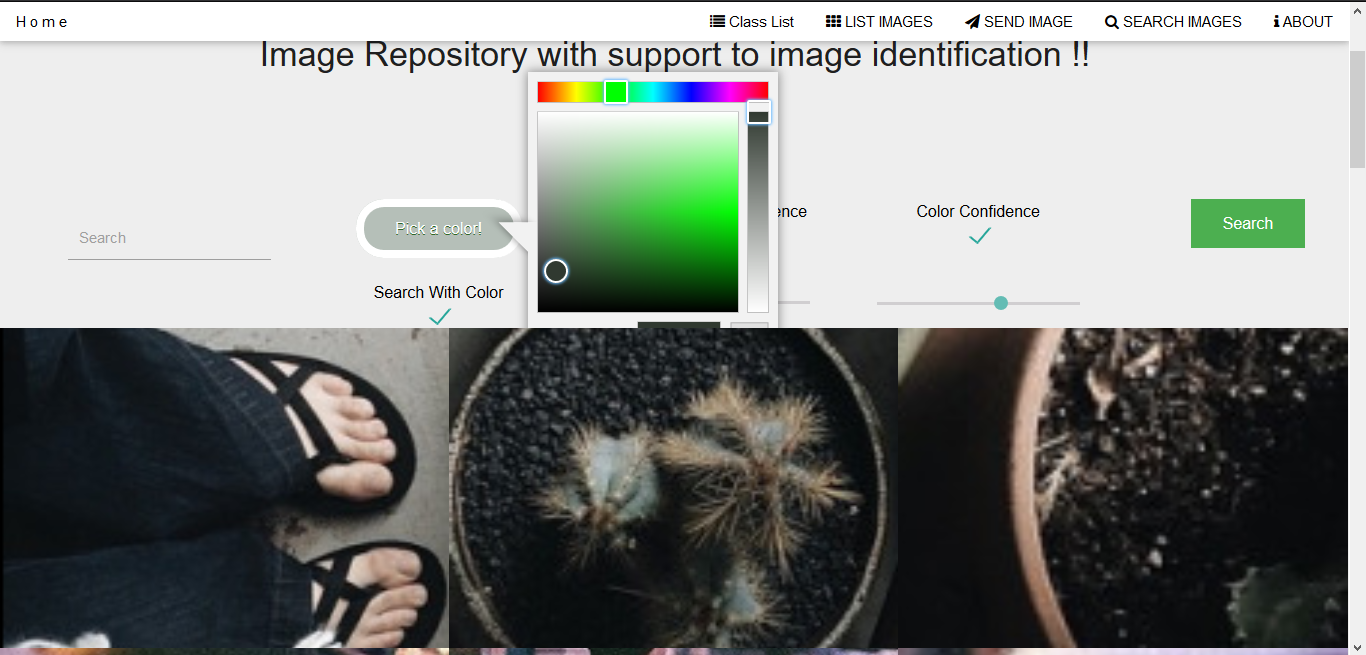
\includegraphics[width=\textwidth]{SearchWithColor.png}
\caption{Página de pesquisa por cor}
\label{Fig7}
\end{figure}

\begin{figure}[h]
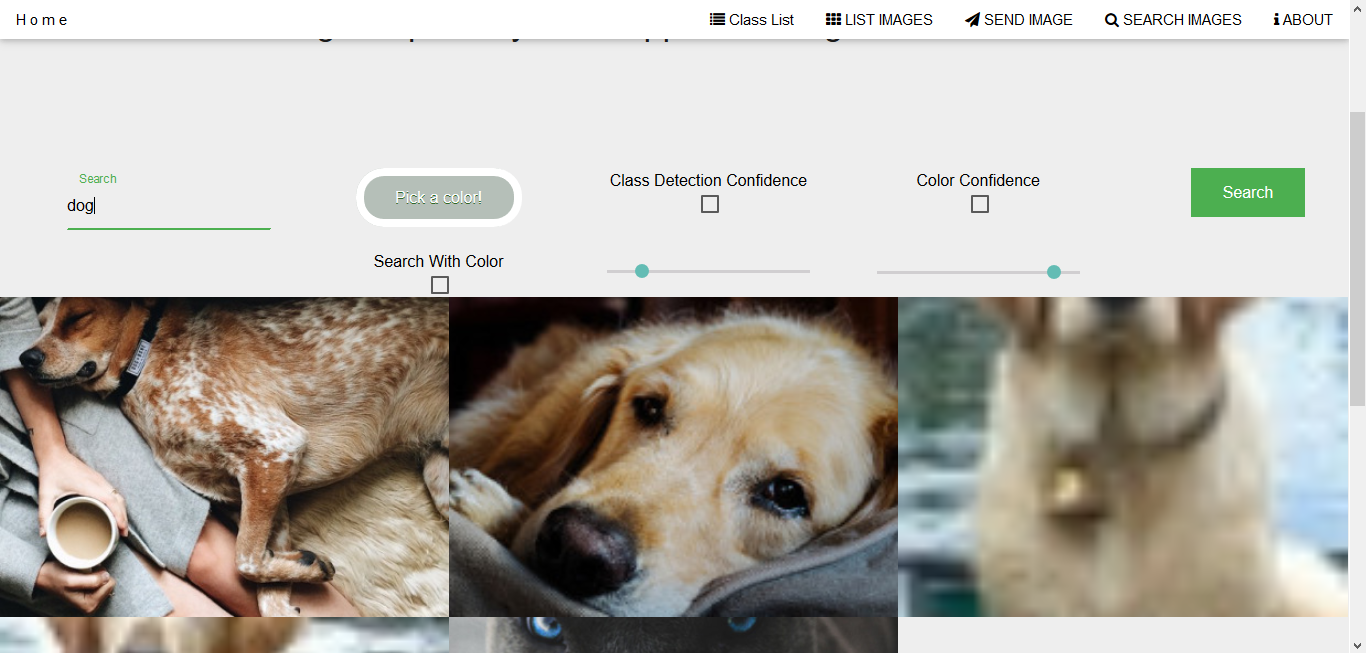
\includegraphics[width=\textwidth]{ClassSearch.png}
\caption{Página de pesquisa por classe}
\label{Fig8}
\end{figure}

\begin{figure}[h]
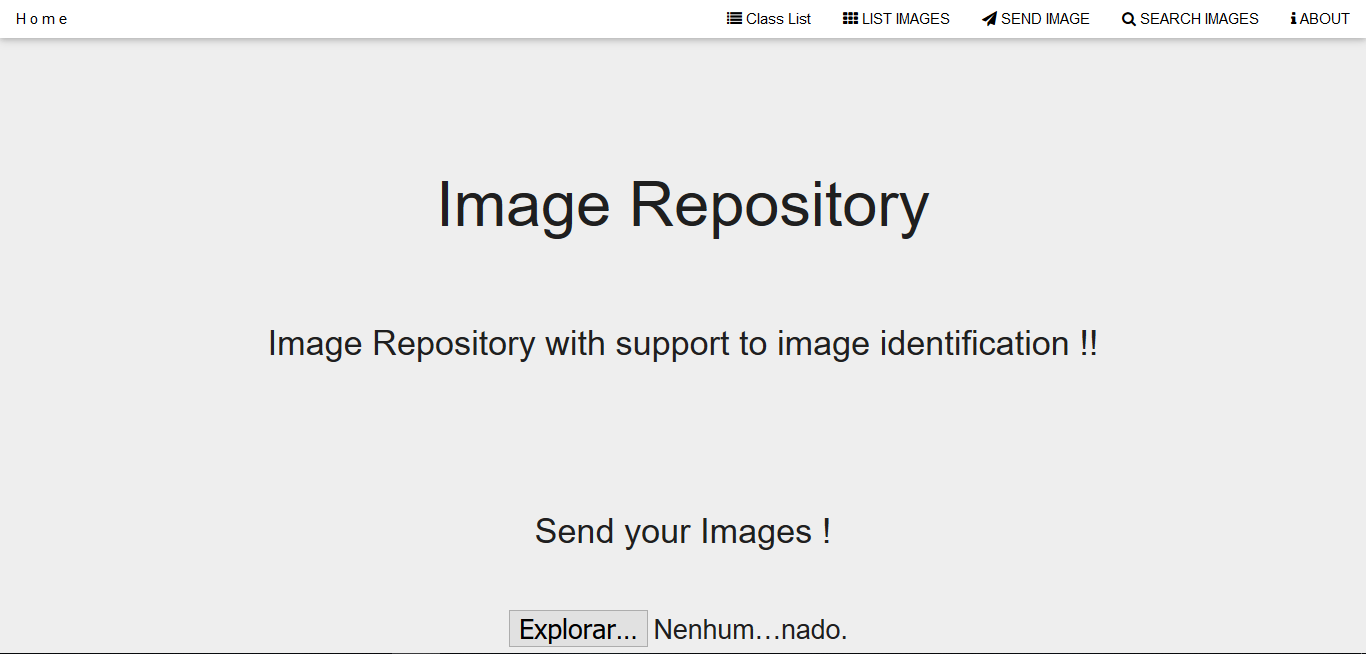
\includegraphics[width=\textwidth]{Send.png}
\caption{Página de submissão de imagens}
\label{Fig9}
\end{figure}

\begin{figure}[h]
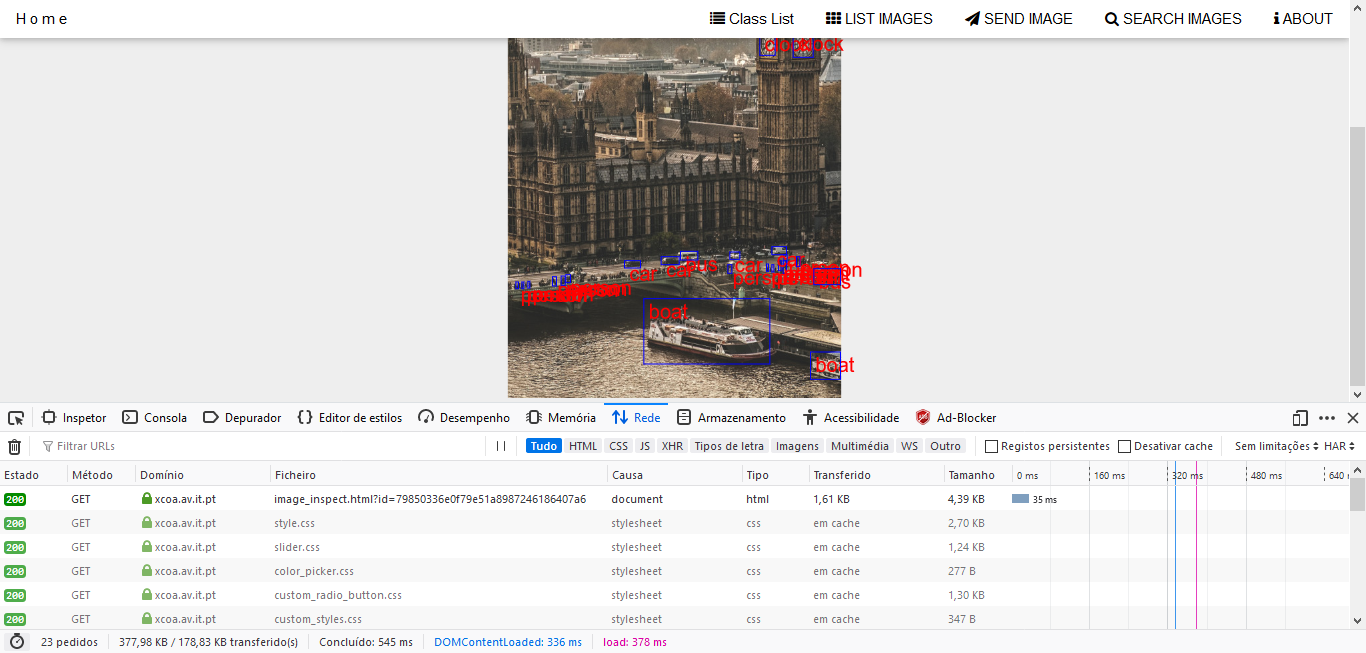
\includegraphics[width=\textwidth]{ResultadosInspect.png}
\caption{Página de inspeção de uma imagem com os vários GET requests}
\label{Fig10}
\end{figure}

\chapter{Análise}
\label{chap.analise}
Analisa os resultados.

\chapter{Conclusões}
\label{chap.conclusao}
Apresenta conclusões.

\chapter*{Contribuições dos autores}
Resumir aqui o que cada autor fez no trabalho.
Usar abreviaturas para identificar os autores,
por exemplo AS para António Silva.
No fim indicar a percentagem de contribuição de cada autor.

%%%%%%%%%%%%%%%%%%%%%%%%%%%%%%%%%
\chapter*{Acrónimos}
\begin{acronym}
\acro{ua}[UA]{Universidade de Aveiro}
\acro{miect}[MIECT]{Mestrado Integrado em Engenharia de Computadores e Telemática}
\acro{lei}[LEI]{Licenciatura em Engenharia Informática}
\acro{glisc}[GLISC]{Grey Literature International Steering Committee}
\acro{HTML}[HTML]{HyperText Markup Language}
\acro{JS}[JS]{JavaScript}
\acro{CSS}[CSS]{Cascading Style Sheets}
\acro{json}[JSON]{JavaScript Object Notation}
\end{acronym}


%%%%%%%%%%%%%%%%%%%%%%%%%%%%%%%%%
\printbibliography

\end{document}
